\section{Evénements}\label{sec:evenements}
\subsection{Composition et exécution de programme}

Un programme est composé de trois parties principales :
\begin{itemize}
    \item \textbf{Code machine} : Instructions représentant la logique des traitements.
    \item \textbf{Espace de données} : Contient les données manipulées par le programme (variables globales, tableaux, variables dynamiques obtenues via \texttt{malloc}).
    \item \textbf{Stack} : Héberge les données de travail courantes (variables locales) et les informations d'appels de fonctions imbriquées.
\end{itemize}

Ces composantes sont liées par des adresses, utilisées pour les branchements, appels et retours de fonction, accès aux cases d'un tableau, et manipulations de la stack. 
Pour s'exécuter, elles doivent être placées en mémoire principale.

Le processeur suit un cycle \textit{fetch-decode-execute} :
\begin{enumerate}
    \item \textbf{Fetch} : Récupération de l'instruction à exécuter depuis la mémoire.
    \item \textbf{Decode} : Décodage des détails de l'instruction pour déterminer le traitement.
    \item \textbf{Execute} : Exécution des opérations requises par l'instruction
    \begin{enumerate}
        \item Mise à jour des registres, de la stack, des données.
        \item Mise à jour (incrément) du Pointeur d'Instruction
    \end{enumerate}
\end{enumerate}

L'\textit{instruction pointer} (ou \textit{program counter}) contient l'adresse de l'instruction courante et est mis à jour après chaque instruction (soit par incrémentation, soit par branchement). 
L'état du programme à un moment donné est déterminé par :
\begin{itemize}
    \item Les valeurs des registres
    \item Le contenu de la stack
    \item Le contenu de l'espace de données
    \item L'\textit{instruction pointer}
\end{itemize}

Une sauvegarde de ces éléments représente un instantané de l'état du programme, permettant de reprendre l'exécution là où elle s'est arrêtée.

\begin{figure}[h]
    \centering
    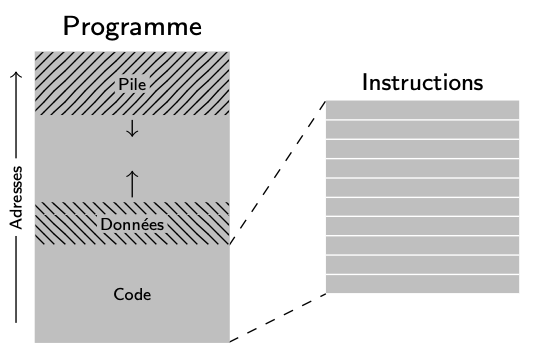
\includegraphics[width=0.4\textwidth]{Images/View/program-view.png}
    \caption{Program view}
\end{figure}

\subsection{Concept de base – évènement}

Lorsqu’un programme est exécuté par le processeur, deux questions se posent :
\begin{itemize}
    \item \textbf{Erreur d'instruction} : Doit-on redémarrer la machine ou gérer l’anomalie pour limiter les dégâts ?
    \item \textbf{Activité de périphérique externe} (e.g. frappe au clavier) : Peut-on suspendre temporairement le programme en cours pour traiter l’activité ?
\end{itemize}

Ces situations sont résolues par la gestion des \textbf{évènements}, mécanismes permettant au processeur de brancher vers du code spécifique en réponse à un évènement.

Les exceptions et interruptions sont des mécanismes implémentés par le processeur permettant d'effectuer un branchement en réaction à un événement.

Les différents types d'événements auxquels un OS peut être confronté sont définis par l'architecture du processeur qui les exécute.

Le système d'exploitation dispose d'un gestionnaire d'événements qui prend le relais en cas d'interruption ou d'exception lors de l'exécution d'un programme.

\subsection{Privilèges}

La vérification du niveau de privilèges est nécessaire pour :
\begin{enumerate}
    \item Modifier la configuration des interruptions/exceptions
    \item Modifier la configuration de la mémoire
    \item Modifier le niveau de privilège courant
\end{enumerate}

Dans une architecture x86, il ya 4 anneaux de protection
\begin{enumerate}
    \item Ring 0: Noyau du os
    \item Ring 1 \& 2 : Services de l'OS
    \item Ring 3 : Programmes
\end{enumerate}

Dans une architecture MIPS, il y a 2 modes de fonctionnement:
\begin{itemize}
    \item Kernel Mode : os
    \item User Mode : programmes
\end{itemize}

\subsection{Typologie}
\subsubsection{Exceptions (évènements synchrones)}
Origine interne, résultant de l’exécution d'une instruction problématique :
\begin{itemize}
    \item \textbf{Code opératoire invalide} : Opcode non reconnu par le processeur.
    \item \textbf{Division par zéro} : Nécessité d’un dénominateur non-nul.
    \item \textbf{Instruction privilégiée} : Niveau de privilège insuffisant pour exécuter l’instruction.
    \item \textbf{Instruction non-chargée en mémoire} : Le système d’exploitation charge la partie manquante en mémoire.
\end{itemize}

\subsubsection{Interruptions (évènements asynchrones)}
Origine externe, provoquées par un signal de périphérique :
\begin{itemize}
    \item \textbf{Frappe de clavier} : Fermeture d’un circuit électronique, générant une interruption.
    \item \textbf{Fichier prêt pour lecture} : Le contrôleur de disque génère une interruption après lecture des données.
    \item \textbf{Réception d’un paquet réseau} : La carte réseau génère une interruption après réception complète d’un paquet.
    \item \textbf{Erreur du matériel} : Anomalies détectées (e.g. température excessive).
    \item \textbf{Signal d’horloge} : Interruption générée 32.768 fois par seconde pour suivre le temps.
\end{itemize}

\subsubsection{Traitements}
Multiplicité des événements (interruptions) => priorité
Evenements pendant le traitement d'évenements (exceptions) => Réantrance et préemption


\subsection{Conséquences possibles pour le programme}

Le système d'exploitation doit gérer les évènements survenus pendant l'exécution d'un programme. 
Selon la nature de l'évènement, deux décisions peuvent être prises :

\begin{itemize}
    \item \textbf{Évènement récupérable} : Après traitement, il est possible de continuer l'exécution du programme.
    \item \textbf{Évènement irrécupérable} : La faute ne peut être corrigée, et il est nécessaire de terminer le programme.
\end{itemize}

\subsubsection{Evenement récupérable}

Lorsqu'un évènement récupérable survient, il est crucial de préserver l'état du processeur. 
Le gestionnaire d'évènements doit sauvegarder le contexte du programme suspendu (registres et stack) avant de traiter l'évènement.
Cette sauvegarde est similaire à celle d'un appel de fonction.

% Le gestionnaire d'évènements sauvegarde uniquement les registres pertinents (e.g. $r_, $s_, $t_). 
% Certaines architectures de processeur utilisent un mécanisme de basculement de stack pour éviter les interférences.

\begin{enumerate}
    \item Sauvegarde
    \item Traitement
    \begin{itemize}
        \item Reprise
        \begin{enumerate}
            \item Identifier
            \item Charger
        \end{enumerate}
        \item Poursuite
        \begin{enumerate}
            \item Récupérer le code
            \item Notifier
            \item Transfert du code vers le programme
        \end{enumerate}
    \end{itemize}
    \item Restauration
    \item La continuation peut être :
    \begin{itemize}
        \item \textbf{Reprise} : Retenter l'exécution de l'instruction qui a causé l'évènement.
        A l'adresse de l'instruction corrélée à cet événement.
        \item \textbf{Poursuite} : Passer à l'instruction suivante.
        A l'adresse de l'instruction suivante.
    \end{itemize}
\end{enumerate}

Les interruptions sont généralement des évènements récupérables avec poursuite, car elles n'affectent pas l'instruction en cours. 
Les exceptions comme les appels systèmes (e.g. \texttt{syscall}, \texttt{int}) sont également des évènements récupérables avec poursuite.

Par exemple, une interruption causée par une frappe au clavier est traitée en lisant le code de la touche depuis un port d'entrée/sortie, le traduisant en caractère, puis le transférant au programme destinataire, souvent la fenêtre active dans une interface graphique.

\subsubsection{Evenement irrécupérable}

Lorsqu'un évènement irrécupérable survient, le programme ne peut plus continuer.
Une sauvegarde complète du contexte d'exécution est effectuée pour le débogage.

Le programme acquiert diverses ressources (mémoire, descripteurs de fichiers, sockets) au cours de son exécution. 
Ces ressources doivent être libérées lorsque le programme est terminé.

\begin{enumerate}
    \item Sauvegarde
    \item Libération des ressources
    \item Traitement
    Les étapes de gestion d'un évènement irrécupérable incluent :
    \begin{itemize}
        \item Affichage d'une notification à l'utilisateur décrivant le problème rencontré.
        \item Sauvegarde du contexte dans un fichier (e.g. \texttt{coredump}) ou envoi par mail à un serveur de rapports de crash.
        \item Libération du processeur, permettant la continuation d'un autre programme via un \textit{context switch}.
    \end{itemize}
    \item Abandon 
\end{enumerate}

\subsection{Mécanismes de déroutement}

Chaque architecture de processeur spécifie et implémente son mécanisme de déroutement pour la gestion des évènements. 
Deux techniques principales sont utilisées :

\begin{itemize}
    \item \textbf{Déroutement avec registre de cause} : Un registre indique la cause de l'évènement, permettant au gestionnaire d'évènements de déterminer l'action appropriée.
    \item \textbf{Vectorisation} : Différents types d'évènements sont associés à des adresses spécifiques dans une table de vecteurs, chaque adresse pointant vers le code de gestion correspondant.
\end{itemize}

La technique utilisée influence l'organisation et les responsabilités du code du gestionnaire d'évènements.


\subsubsection{Registre de cause}

Le registre de cause encode les évènements survenus lors du cycle d’exécution courant, mettant à jour les bits pour les exceptions et interruptions. 
Si au moins un bit est positionné, le processeur réalise un déroutement vers une adresse précise.

Le gestionnaire d’évènements doit :
\begin{itemize}
    \item Lire le contenu du registre de cause.
    \item Tester et traiter les bits des interruptions en attente (bits à 1).
    \item Traiter les exceptions stipulées par le code d’exception.
\end{itemize}

Cette technique permet au système d’exploitation de déterminer l’ordre de priorité des traitements des différents évènements. 
La fonction principale du gestionnaire d’évènements doit être placée à l’adresse de déroutement définie par le processeur au démarrage du système.

Pour permettre la continuation du programme, l’adresse de l’indicateur d’instruction courante est sauvegardée dans un registre dédié (e.g. Exception Program Counter en MIPS32).


\subsubsection{Vectorisation}

Dans la vectorisation, chaque type d'évènement est associé à un numéro unique (e.g. interrupt vector). 
Ce numéro identifie une entrée dans une table de descripteurs (e.g. interrupt descriptor table, IDT) qui référence la fonction de traitement spécifique à invoquer (interrupt service routine, ISR).

À la fin d’un cycle d’exécution, le processeur :
\begin{itemize}
    \item Consulte les numéros d’évènements survenus.
    \item Invoque les fonctions de gestion des évènements correspondantes dans un ordre déterminé.
\end{itemize}

Le code du gestionnaire d’évènements se concentre uniquement sur l’évènement correspondant. 
Au démarrage du système, l’OS initialise le contenu de la table des descripteurs et la référence au processeur via une instruction privilégiée (e.g. \texttt{lidt} en x86).

Lorsqu’un évènement survient :
\begin{itemize}
    \item Le numéro d’évènement sert d’indice dans l’IDT.
    \item Le descripteur correspondant (interrupt gate) contient l’adresse de la fonction de gestion vers laquelle brancher (offset).
\end{itemize}


\subsubsection{Niveaux de privilège}

Le jeu d'instructions d'un processeur inclut toutes les instructions reconnaissables par son architecture, comprenant les instructions arithmétiques, logiques et systèmes.
Les instructions systèmes modifient la configuration du processeur et doivent être exécutées uniquement par le système d'exploitation.

Un niveau de privilège contrôle quelles instructions peuvent être exécutées et quand. 
La spécification du processeur décrit la dynamique de changement de ce niveau de privilège et son utilisation pour les vérifications. 

\subsubsection{Basculement de stack}

Lorsqu’un évènement survient, le processeur déroute vers une fonction du système d’exploitation, modifiant le contenu des registres et utilisant une stack pour stocker les valeurs temporaires. 
Il est crucial de décider si cette stack sera celle du programme suspendu ou une stack dédiée du système d’exploitation.

Le processeur peut basculer vers une stack du système d’exploitation, en sauvegardant les informations nécessaires pour explorer la stack du programme suspendu (e.g. stack pointer). 
Par exemple, lors d'un appel système, les arguments peuvent être passés via la stack, et le système d’exploitation doit pouvoir les localiser.

Après le traitement de l’évènement, la stack courante redevient celle du programme. 
La figure 1.11 illustre ce processus :
\begin{itemize}
    \item Avant le déroutement : \texttt{sp(pgm)}
    \item Après le déroutement : \texttt{sp(os)}, contenant :
    \begin{itemize}
        \item Sauvegarde du pointeur de stack précédent \texttt{sp(pgm)}
        \item Indicateur d’instruction courante \texttt{ip(pgm)}
        \item Éventuel code d’erreur décrivant l’évènement
    \end{itemize}
\end{itemize}

Ces informations permettent de revenir au programme pour une éventuelle continuation.



\subsection{Multiplicité des occurences}

Il est possible que plusieurs évènements se produisent pendant un même cycle d’exécution du processeur. 
Les règles d'agrégatioons entre événements sont les suivantes :

\begin{itemize}
    \item \textbf{Reprise} l’emporte sur une \textbf{poursuite}.
    \item \textbf{Abandon} l’emporte sur une \textbf{reprise}.
\end{itemize}

Lors de deux évènements similaires (deux poursuites, deux reprises, ou deux abandons), la conséquence est respectivement une poursuite, une reprise, ou un abandon.

Pour des évènements de types différents :
\begin{itemize}
    \item \textbf{Reprise et poursuite} : La reprise l’emporte, les deux traitements doivent être réalisés. 
    Si l'évènement avec poursuite est une interruption, il peut être traité en priorité.
    \item \textbf{Poursuite et abandon} : L’abandon l’emporte. Si l'évènement avec poursuite est une exception, son traitement n'est pas nécessaire. 
    Si c'est une interruption, il doit être traité.
    \item \textbf{Reprise et abandon} : L’abandon l’emporte. Le traitement de l'évènement avec reprise n'est pas nécessaire car le programme ne continuera plus.
\end{itemize}



\subsection{Gestion ré-entrante des évènements}

Un évènement peut survenir pendant n'importe quel cycle d'exécution, y compris pendant la gestion d'un autre évènement (exception ou interruption). 
Le gestionnaire d'évènements doit être adapté pour gérer cette imbrication correctement.

Un gestionnaire ré-entrant permet de gérer de nouveaux évènements survenant pendant l'exécution du gestionnaire actuel. 
Les considérations sont similaires à la gestion des appels de fonctions récursives. 

Pour garantir une sauvegarde cohérente des contextes imbriqués :
\begin{itemize}
    \item Utiliser la stack pour sauvegarder le contexte du gestionnaire d'évènements suspendu.
    \item Désactiver les interruptions pendant les phases critiques (sauvegarde du contexte, restauration du contexte, continuation), mettant ainsi en attente les interruptions.
    \item Préserver l'adresse de l'instruction corrélée à chaque niveau d'imbrication.
\end{itemize}

\subsection{Priorités et masques d'interruptions}

Dans un système typique, il est crucial de respecter l'ordre de priorité des interruptions. 
Un gestionnaire ré-entrant seul ne suffit pas pour éviter l'inversion de priorité, où une interruption de basse priorité pourrait interrompre le traitement d'une interruption de haute priorité.

La solution consiste à utiliser un masque d'interruptions, permettant une granularité dans l'activation et la désactivation des interruptions. 
Ce masque contrôle quelles interruptions sont actives (ou inactives) en utilisant un bit par type d'interruption. 
Le masque est combiné avec les bits des interruptions en attente à la fin de chaque cycle d'exécution.

Lors du traitement d'une interruption, le gestionnaire :
\begin{itemize}
    \item Positionne les bits du masque pour autoriser uniquement les interruptions plus prioritaires.
    \item Après traitement, restaure l'état du masque à son état précédent.
\end{itemize}

